\subsubsubsection{Registrovanje klijenta}

\begin{itemize}
    \item Kratak opis:
        \begin{itemize}
            \item Potencijalni klijent se kroz aplikaciju registruje kako bi mogao da koristi usluge HelloFresh.
        \end{itemize}
    \item Učesnici:
        \begin{itemize}
            \item Potenijalni klijent koji želi da koristi usluge HelloFresh aplikacije.
        \end{itemize}
    \item Preduslovi:
        \begin{itemize}
            \item Mejl adresa klijenta ne postoji u sistemu
        \end{itemize}
    \item Postuslovi:
        \begin{itemize}
            \item Potencijalni klijent je registrovana kao aktivni klijent HelloFresh aplikacije.
        \end{itemize}
    \item Osnovni tok:
        \begin{enumerate}
            \item Potencijalni klijent pristupa veb stranici i otvara formu za registraciju.
            \item Potencijalni klijent popunjava formu za registraciju.
            \item Potencijalni klijent potvrđuje svoju registraciju.
            \item Sistem vrši validaciju registracije.
            \item Sistem pamti unetu registraciju.
            \item Sistem šalje mejl klijentu o uspešnoj registraciji i pravilima korišnjenja naloga.
        \end{enumerate}
    \item Alternativni tok:
        \begin{itemize}
            \item[3.a] Potencijalni klijent odustaje od registracije. Slučaj upotrebe se završava.
            \item[4.a] Ukoliko je potencijalni klijent odabrao korisničko ime koje već postoji u sistemu, prikazuje se odgovarajuća poruka. Slučaj upotrebe se nastavlja od koraka 2.
            \item[4.b] Ukoliko je potencijalni klijent odabrao lozinku koja ne odgovara specifikacijama sistema (prekratka), prikazuje se odgovarajuća poruka. Slučaj upotrebe se nastavlja od koraka 2.
        \end{itemize}
    \item Dodatne informacije:
    \begin{itemize}
        \item Forma za registraciju sadrži sledeće podatke: korisničko ime, lozinka, mejl adresa
    \end{itemize}
\end{itemize}

\begin{figure}[H]
\begin{center}
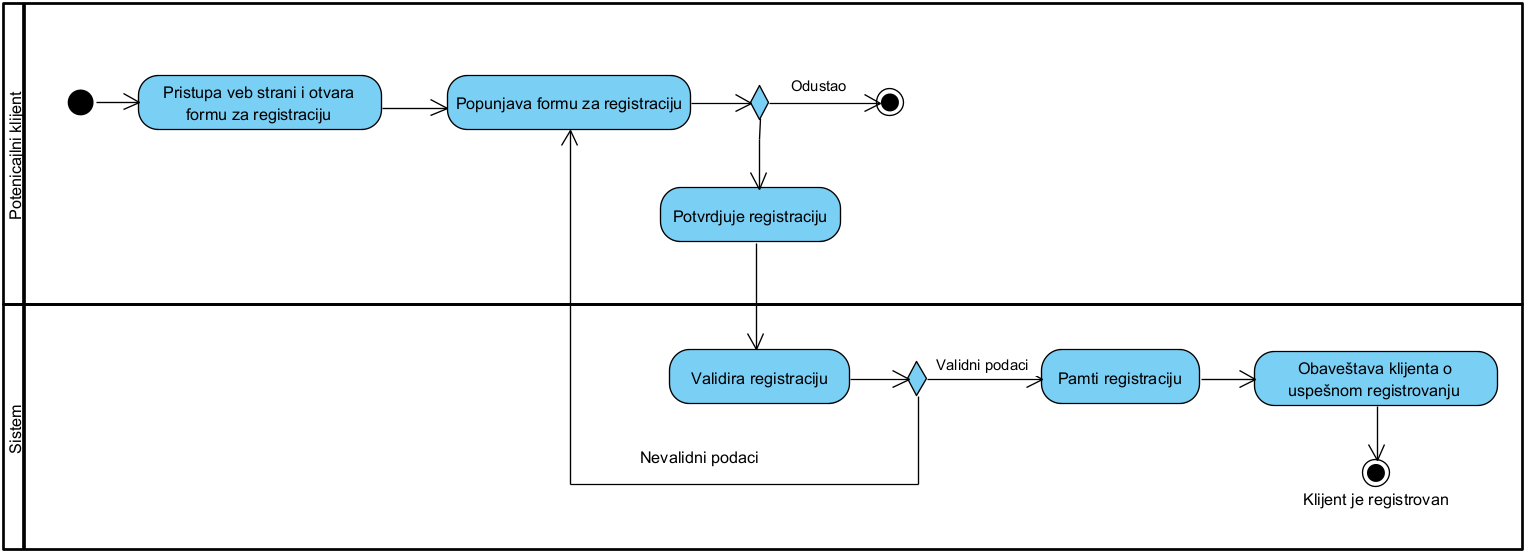
\includegraphics[width=\textwidth]{Pictures/activity_client_registration.png}
\end{center}
    \caption{Dijagram aktivnosti registrovanja potencijalnog klijenta}
\label{fig:ActivityClientRegistration}
\end{figure}
